Sei \(\mathcal{M}^n\) eine Mannigfaltigkeit und \({n=i+j+1}\). Chirurgie ist der Prozess, \(\mathcal{M}\) mit der Standardsph\"are \(\mathbb{S}^n\) entlang einer in das Innere von \(\mathcal{M}\) eingebetteten Sph\"are mit trivialem Normalenb\"undel \({\mathbb{S}^i\hookrightarrow\mathring{\mathcal{M}}}\) zu verkleben. Dieser Prozess l\"asst sich auch derart beschreiben, dass eine eingebettete Untermannigfaltigkeit \({\mathbb{S}^i\times\mathbb{D}^{j+1}}\) herausgeschnitten, und die resultierende Mannigfaltigkeit entlang \({\mathbb{S}^i\times\mathbb{S}^j}\) mit \({\mathbb{D}^{i+1}\times\mathbb{S}^j}\) verklebt wird. Dies f\"uhrt zu einer kontrollierten Ver\"anderung der Homologie.

\section{Definitionen}
    Sei \(\mathcal{S}^i\hookrightarrow\mathring{\mathcal{M}}\) eine eingebettete Sph\"are mit trivialem Normalenb\"undel. Die letzte Forderung bedeutet hierbei, dass \({N\mathcal{S}\cong\underline{\mathbb{R}}^{j+1}}\) gilt, sodass eine Tubenumgebung von \(\mathcal{S}\) zu \(\underline{\mathbb{R}}^{j+1}\) isomorph ist. Als Anklebeabbildung sei also eine Einbettung \(\Phi\colon\underline{\mathbb{R}}^{j+1}\hookrightarrow\mathring{\mathcal{M}}\) gew\"ahlt. Da das Normalenb\"undel der eingebetteten Sph\"are \({\mathbb{S}^i\times\{0\}^j\subset\mathbb{S}^n}\) ebenso trivial ist, lassen sich \(\mathcal{M}\) und \(\mathbb{S}^n\) entlang \(\mathcal{S}\cong\mathbb{S}^i\) verkleben. Die entstehende Mannigfaltigkeit gehe durch \textbf{Chirurgie} an \(\mathcal{S}\) aus \(\mathcal{M}\) hervor. Die g\"angigste Bezeichnung ist hierbei wohl \(\chi(\mathcal{M},\Phi)\). Im Folgenden sei stattdessen
\[\mathcal{M}\multimap\mathbb{S}^i:=\mathcal{M}\mathop{+}^{\Phi}\mathbb{S}^n=\chi(\mathcal{M},\Phi)\]
eben jene Chirurgie.
\section{Verbindung zu Henkeln}
    Ein nah mit Chirurgie verbundener Vorgang ist das Anbringen eines Henkels. Sei hierzu \(\mathcal{W}^{n+1}\) eine Mannigfaltigkeit und \(\mathcal{S}^i\hookrightarrow\partial\mathcal{W}\) eine eingebettete Sph\"are mit trivialem Normalenb\"undel in \(\mathcal{W}\). Erneut ist \(N\mathcal{S}\cong\underline{\mathbb{R}}^{n+1}\) (nicht \(\underline{\mathbb{R}}^n\times\mathbb{R}_+\)). Eine Tubenumgebung ist also eine Einbettung \(\tilde{\Phi}\colon\underline{\mathbb{R}}^n\times\mathbb{R}_+\hookrightarrow\mathcal{W}\), die eine Tubenumgebung \(\Phi\colon\underline{\mathbb{R}}^n\hookrightarrow\partial\mathcal{W}\) fortsetzt. Analoges gilt f\"ur \(\mathbb{S}^i\subset\partial\mathbb{D}^{n+1}\). Die Verklebung 
    \[\mathcal{W}\multimap\mathbb{D}^{i+1}:=\mathcal{W}\mathop{+}^{\tilde{\Phi}}\mathbb{D}^{n+1}\,,\]
    gehe durch das \textbf{Anbringen eines Henkels} an \(\mathcal{S}\) aus \(\mathcal{W}\) hervor. Dieser Vorgang geschieht immer am Rand einer Mannigfaltigkeit. Naheliegenderweise gilt
    \[\partial(\mathcal{W}\multimap\mathbb{D}^{i+1})=\partial(\mathcal{W}\mathop{+}^{\tilde{\Phi}}\mathbb{D}^{n+1})\cong\partial\mathcal{W}\mathop{+}^{\Phi}\partial\mathbb{D}^{n+1}=\partial\mathcal{W}\multimap\mathbb{S}^i\,,\]
    der Rand der Anbringung eines Henkels an \(\mathcal{W}\) ist also die Chirurgie an \(\partial\mathcal{W}\). Diese Konstruktion sei in Abbildung \ref{fig:surgery} verdeutlicht. Dies vereinfacht die Sitation f\"ur geschlossene Mannigfaltigkeiten \(\mathcal{M}\), da in diesem Fall \(\mathcal{M}\times\mathbb{I}\) eine \((n+1)\)-Mannigfaltikeit mit \(\partial\mathcal{W}\cong\mathcal{M}\sqcup(-\mathcal{M})\) ist. Es gilt also auch
    \[\partial(\mathcal{M}\times\mathbb{I}\multimap\mathbb{D}^{i+1})\cong\mathcal{M}\sqcup-(\mathcal{M}\multimap\mathbb{S}^i)\]
    sodass \(\mathcal{M}\multimap\mathbb{S}^i\) und \(\mathcal{M}\) kobordant sind. Der Trick die Chirurgie derart als Rand darzustellen vereinfacht einige \"Uber\-le\-gun\-gen. Es sei jedoch Obacht geboten, da \(\mathcal{M}\times\mathbb{I}\) f\"ur glatte Mannigfaltigkeiten \(\mathcal{M}\) mit nicht leerem Rand keine glatte Mannigfaltigkeit ergibt. Entlang der Strata \(\partial\mathcal{M}\times\partial\,\mathbb{I}\) l\"asst sich keine glatte Struktur angeben, die mit der glatten Struktur von \(\mathcal{M}\) \"ubereinstimmt. Da im Folgenden ledliglich Mannigfaltigkeiten \(\mathcal{M}\) betrachtet werden, deren Rand leer oder eine Homotopiesph\"are ist, kann dem folgenderma\ss en Abhilfe geschaffen werden.
    \begin{figure}
    \centering
    \begin{tikzpicture}[scale = 0.6]

        \path (-50:3) arc (-50:230:3)
        \foreach\i in {0, 0.05, 0.1, 0.15, 0.2, 0.25, 0.3, 0.35, 0.4, 0.45, 0.5, 0.55, 0.6, 0.65, 0.7, 0.75, 0.8, 0.85, 0.9, 0.95, 1} { node [pos = \i] (A\i) {}};

        % Right tube backframe
        \foreach\i in {0, 0.05, 0.1, 0.15, 0.2, 0.25, 0.3, 0.35, 0.4, 0.45} { 
            \draw [thick, densely dotted, rotate = -50 + \i * 280] ({A\i}.center) ++(180:1 and 0.5) arc (180:360:1 and 0.3 - 0.875 * \i);
        }
        % Right core
        \draw [thick, orange]
            (-50:3) node {\tiny\textbullet} arc (-50:90:3);

        % Small ball
        \begin{scope}[yshift = 3cm] 
            % Cocore
            \draw [fill, color = darkgreen, opacity = 0.5] (0:0.1375 and 1) arc (0:360:0.1375 and 1);
            % Transversal sphere
            \draw [thick, densely dotted, color = {rgb,255:red,0;green,100;blue,0}] 
                (90:0.1375 and 1) arc (90:270:0.1375 and 1);
            \draw
                (1, 0) arc (0:360:1)
                (180:1 and 0.5) arc (180:360:1 and 0.5);
            \draw [densely dotted]
                (0:1) arc (0:180:1 and 0.5);
        \end{scope}

        % Right tube topframe
        \foreach\i in {0, 0.05, 0.1, 0.15, 0.2, 0.25, 0.3, 0.35, 0.4} { 
            \draw [thick, rotate = -50 + \i * 280] ({A\i}.center) ++(0:1 and 0.5) arc (0:180:1 and 0.3 - 0.875 * \i);
        }

        \path [thick, rotate = -50, color = red] ({A0}.center) ++(0:1 and 0.5) arc (0:180:1 and 0.3) node [pos = 0.7] {\tiny\textbullet};

        % Right tube
        \draw [thick]
            (-50:4) arc (-50:90:4) 
            (-50:2) arc (-50:90:2);

        % Big ball
        \begin{scope}[yshift = -3.75cm, scale = 3]
            \draw [densely dotted]
                (90:0.5 and 1) arc (90:270:0.5 and 1) 
                (0:1 and 0.5) arc (0:180:1 and 0.5);
            \shade[ball color = blue!10!white, opacity = 0.5] (1, 0) arc (0:360:1) -- cycle;
            \draw [thick]
                (0:1) arc (0:360:1) 
                (-90:0.5 and 1) arc (-90:90:0.5 and 1) 
                (180:1 and 0.5) arc (180:360:1 and 0.5);
        \end{scope}

        % Left tube
        \draw [thick]
            (90:4) arc (90:230:4) 
            (90:2) arc (90:230:2);

        % Left tube backframe
        \foreach\i in {0.55, 0.6, 0.65, 0.7, 0.75, 0.8, 0.85, 0.9, 0.95} { 
            \draw [thick, densely dotted, rotate = -50 + \i * 280] ({A\i}.center) ++(0:1 and 0.5) arc (0:180:1 and 0.3 - 0.875 * \i);
        }
        % Meridian backframe
        \draw [thick, densely dotted, rotate = -50 + 280, color = blue] ({A1}.center) ++(0:1 and 0.5) arc (0:180:1 and 0.3 - 0.875) node [pos = 0.6, red] {\tiny\textbullet};
        % Left core
        \draw [thick, orange]
            (90:3) arc (90:230:3) node {\tiny\textbullet};
        
        % Small ball shading
        \shade[ball color = blue!10!white, opacity = 0.5, yshift = 3cm] (1, 0) arc (0:360:1) -- cycle;
        
        % Transversal sphere top frame
        \draw [thick, color = darkgreen, yshift = 3cm] 
            (-90:0.1375 and 1) arc (-90:90:0.1375 and 1);

        % Last right tube topframe 
        \draw [thick, rotate = -50 + 0.45 * 280] ({A0.45}.center) ++(0:1 and 0.5) arc (0:180:1 and 0.3 - 0.875 * 0.45);

        % Left tube topframe
        \foreach\i in {0.55, 0.6, 0.65, 0.7, 0.75, 0.8, 0.85, 0.9, 0.95} { 
            \draw [thick, rotate = -50 + \i * 280] ({A\i}.center) ++(180:1 and 0.5) arc (180:360:1 and 0.3 - 0.875 * \i);
        }
        % Meridian topframe
        \draw [thick, rotate = -50 + 280, color = blue] ({A1}.center) ++(180:1 and 0.5) arc (180:360:1 and 0.3 - 0.875);
        
    \end{tikzpicture}
    \caption{Eine Vollkugel mit einem Henkel. Farblich markiert sind \textcolor{orange}{Kern}, \textcolor{darkgreen}{Kokern}, \textcolor{blue}{Meridian} und \textcolor{red}{\"Aquator}.}\label{fig:surgery}
\end{figure}
    \newpage
    \begin{lemma}\label{lem:smooth_man}
        Zu jeder Mannigfaltigkeit \(\mathcal{M}^n\) existiert eine Mannigfaltigkeit
        \[\mathcal{W}^{n+1}\subseteq\mathcal{M}\times\mathbb{I}\quad\text{mit}\quad\partial\mathcal{W}\cong\mathcal{M}\mathop{+}^{\partial\mathcal{M}}\mathcal{M}\,.\]
    \end{lemma}
    \begin{proof}
        Eine Kragenumgebung von \(\partial\mathcal{M}\) in \(\mathcal{M}\) kann zu einer topologischen Einbettung \(\partial\mathcal{M}\times\mathbb{R}_+^2\hookrightarrow\mathcal{M}\times\mathbb{I}\) fortgesetzt werden. Dann kann \(\mathbb{R}_+^2\) durch eine geeignete glatte Mannigfaltigkeit mit Rand ersetzt werden. Eine M\"oglichkeit diese zu definieren w\"are als jenes Gebiet \(Q\subseteq\mathbb{R}_+^2\), welches durch die Kurve \(\gamma\) abgegrenzt wird, die durch
        \[\gamma(t):=\left(1+t^2\right)\left(\cos(g(t)),\sin(g(t))\right)\quad\text{mit}\quad g(t)=\frac{h\left(t+\frac{1}{2}\right)}{h\left(t+\frac{1}{2}\right)+h\left(\frac{1}{2}-t\right)}\]
        und
        \[h(t)=\begin{cases}
            e^{-\frac{1}{x}} & x\geq0\\
            0 & \text{sonst}
        \end{cases}\]
        definiert ist. Siehe hierzu Abbildung \ref{fig:smooth_man}. Bezeichne die resultierende Mannigfaltigkeit durch \(\mathcal{W}\). Der Rand dieser Gl\"attung ist gerade eine Gl\"attung von
        \[\partial(\mathcal{M}\times\mathbb{I})=\partial\mathcal{M}\times\mathbb{I}\cup\mathcal{M}\times\partial\,\mathbb{I}\,.\]
        Aus der Definition l\"asst sich erkennen, dass diese zu \(\mathcal{M}+_{\partial\mathcal{M}}\mathcal{M}\) diffeomorph ist.
    \end{proof}
    \begin{figure}
        \centering
        \includegraphics[scale = 2]{Kapitel/Chirurgie/geogebra-export.png}
        \caption{Eine glatte Kurve, sodass das oben rechts berandete Gebiet eine glatte Mannigfaltigkeit mit Rand ist, die zum \(\mathbb{R}_+^2\) hom\"oomorph ist.}\label{fig:smooth_man}
    \end{figure}
    Sei \(\mathcal{W}\) gem\"a\ss{} Lemma \ref{lem:smooth_man}. Wird ein Henkel an dem Rand von \(\partial\mathcal{W}\) angebracht, ergibt sich
    \[\partial\left(\mathcal{W}\multimap\mathbb{D}^{i+1}\right)\cong\mathcal{M}\mathop{+}^{\partial\mathcal{M}}\left(\mathcal{M}\multimap\mathbb{S}^i\right)\,.\]
    Wenn \(\partial\mathcal{M}\) zus\"atzlich leer oder eine Homotopiesph\"are ist, folgt f\"ur \(0<i<n\) 
    \[H_i(\partial\mathcal{W})\cong H_i(\mathcal{M})\oplus H_i(\mathcal{M})\,.\]
    Diese Mannigfaltigkeit verh\"alt sich deshalb \"ahnlich genug zu \(\mathcal{M}\times\mathbb{I}\).

\subsection{Kombinatorische Chirurgie}
    Besonders im Rahmen homologischer \"Uberlegungen ist die glatte Struktur der Mannigfaltigkeit nicht vonn\"oten, sodass in diesem Fall eine topologisch \"aqui\-va\-len\-te und einfachere Notation genutzt werden kann. Sei eine glatte Einbettung \(\Phi\colon\mathbb{S}^i\times\mathbb{D}^{j+1}\hookrightarrow\mathring{\mathcal{M}}\) mit \(\mathcal{D}:=\im\Phi\) gegeben. Setze \(\mathcal{M}_0:=\mathcal{M}\setminus\mathring{\mathcal{D}}\) und betrachte das topologische Pushout
    \[\mathcal{M}^{\prime}:=\mathcal{M}_0\cup_{\partial\mathcal{D}}\left(\mathbb{D}^{i+1}\times\mathbb{S}^j\right)\,.\]
    Ebenso l\"asst sich das Anbringen eines Henkels an \(\mathcal{W}^{n+1}\) durch
    \[\mathcal{W}+H^i:=\mathcal{W}\cup_{\mathcal{D}}\left(\mathbb{D}^{i+1}\times\mathbb{D}^{j+1}\right)\]
    definieren. Die entstehende Mannigfaltigkeit sind hierbei hom\"oomorph zu ihren oberen glatten Definitionen (\cite{kosinski1992differential} Kapitel VI Proposition 8.1). 
    
    \subsubsection{Meridian und \"Aquator einer Chirurgie}
        Diese Definition legt nahe, warum \(\mathbb{S}^i\times\mathbb{S}^j\) bei dem Untersuchen von einer Chirurgie eine wichtige Rolle spielt. F\"ur ein \(x\in\mathbb{S}^i\) und ein \(y\in\mathbb{S}^j\) sei \(\Phi\left(\{x\}\times\mathbb{S}^j\right)\) ein \textbf{Meridian} und \(\Phi\left(\mathbb{S}^i\times\{y\}\right)\) ein \textbf{\"Aquator}. 

    \subsubsection{Kern und Kokern eines Henkels}
        Der Anteil von \(\mathcal{W}\multimap\mathbb{D}^{i+1}\), der mit \(\mathbb{D}^{i+1}\times0\) korrespondiert hei\ss e \textbf{Kern} und der Anteil \(0\times\mathbb{D}^{j+1}\) hei\ss e \textbf{Kokern}. Der Rand des Kernes ist gerade die Anklebesph\"are, der Rand des Kokerns hei\ss e transversale Sph\"are. Diese Begriffe sind insbesondere im Rahmen des H-Kobordismus-Satzes wichtig.


\section{Chirurgie unterhalb mittlerer Dimension}
    Der Effekt einer Chirurgie auf die niederen Homologiegruppen ist recht simpel. Sei \(n=i+j+1\), \(\mathcal{M}^n\) eine Mannigfaltigkeit, \(\mathcal{S}^i\hookrightarrow\mathcal{M}\) eine eingebettete Sph\"are mit trivialem Normalenb\"undel und \(\Phi\colon\underline{\mathbb{D}}^{j+1}\hookrightarrow\mathcal{M}\) eine zugeh\"orige Anklebeeinbettung. Setze \(\mathcal{D}:=\im\Phi\) und
\[\mathcal{M}_0:=\mathcal{M}\setminus\mathring{\mathcal{D}}\quad\text{sowie}\quad\mathcal{M}^{\prime}:=\mathcal{M}_0\cup_{\partial\mathcal{D}}\left(\mathbb{D}^{i+1}\times\mathbb{S}^j\right)\,.\] 
Dann lassen sich die langen exakten Folgen der Paare \((\mathcal{M},\mathcal{M}_0)\) und \((\mathcal{M}^{\prime},\mathcal{M}_0)\) zu folgendem Diagramm zusammensetzen:
\begin{center}
    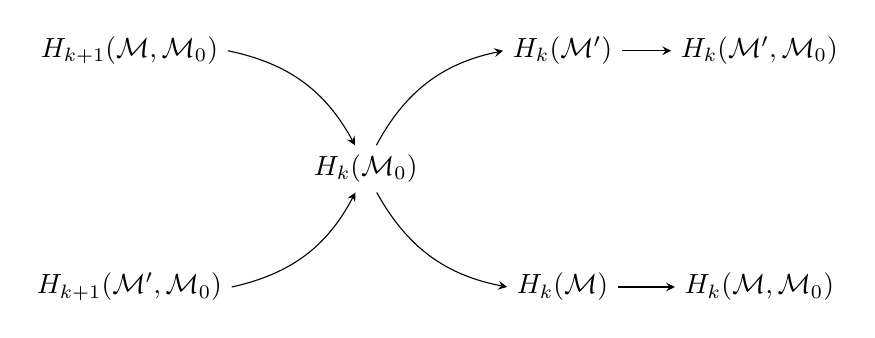
\begin{tikzpicture}
        \draw
            (-3, -1.5) node (B) {\(H_{k+1}(\mathcal{M}^{\prime},\mathcal{M}_0)\)}
            (0, 0) node (C) {\(H_k(\mathcal{M}_0)\)}
            (2.5, 1.5) node (D) {\(H_k(\mathcal{M}^{\prime})\)}
            (5, 1.5) node (E) {\(H_k(\mathcal{M}^{\prime},\mathcal{M}_0)\)}
            (-3, 1.5) node (G) {\(H_{k+1}(\mathcal{M},\mathcal{M}_0)\)}
            (2.5, -1.5) node (H) {\(H_k(\mathcal{M})\)}
            (5, -1.5) node (I) {\(H_k(\mathcal{M},\mathcal{M}_0)\)}
            
            (B.east) edge [bend right = 25, -stealth] (C)
            (C) edge [bend left = 25, -stealth] (D.west)
            (D) edge [-stealth] (E)

            (G.east) edge [bend left = 25, -stealth] (C)
            (C) edge [bend right = 25, -stealth] (H.west)
            (H) edge [-stealth] (I)
            ;
    \end{tikzpicture}
\end{center}
Per Ausschneidung folgen
\[H_k(\mathcal{M},\mathcal{M}_0)\cong H_k(\mathbb{S}^i\times\mathbb{D}^{j+1},\mathbb{S}^i\times\mathbb{S}^j)\cong\begin{cases}
    \mathbb{Z} & k\in\{0,j+1\}\\
    0 & 0<k<j+1
\end{cases}\]
und 
\[H_k(\mathcal{M}^{\prime},\mathcal{M}_0)\cong H_k(\mathbb{D}^{i+1}\times\mathbb{S}^j,\mathbb{S}^i\times\mathbb{S}^j)\cong\begin{cases}
    \mathbb{Z} & k\in\{0,i+1\}\\
    0 & 0<k<i+1
\end{cases}\,.\]
F\"ur die Berechnung siehe Appendix. Die Erzeuger der \(\mathbb{Z}\)-Anteile in Dimension \(i+1\) und \(j+1\) sind gerade die Bilder der Erzeuger von \(H_{i+1}(\mathbb{D}^{i+1},\mathbb{S}^i)\) und \(H_{j+1}(\mathbb{D}^{j+1},\mathbb{S}^j)\) und stehen somit in Korrespondenz zu Fundamentalklassen eines \"Aquators \(e=\Phi(x\times\mathbb{S}^j)\) und einem Meridian \(m=\Phi(\mathbb{S}^i\times y)\). \"Aquator und Meridian sind deswegen interessant, da sie beide in \(\mathcal{M}_0\) liegen, und die Beziehungen
\[\eqcl{e\mathrel{|}\mathcal{M}}=\eqcl{\mathcal{S}\mathrel{|}\mathcal{M}},\quad\eqcl{m\mathrel{|}\mathcal{M}}=0\quad\text{sowie}\quad\eqcl{e\mathrel{|}\mathcal{M}^{\prime}}=0\]
erf\"ullen. Die Sph\"are hei\ss e \textbf{primitiv}, wenn ein \(g\in H_j(\mathcal{M})\) mit \(g\cdot\eqcl{\mathcal{S}\mathrel{|}\mathcal{M}}=1\) existiert.
\begin{lemma}
    Chirurgie an einer Sph\"are \(\mathcal{S}^i\hookrightarrow\mathcal{M}^n\) mit \(i<j\) eliminiert die Fundamentalklasse \(\eqcl{\mathcal{S}\mathrel{|}\mathcal{M}}\).
\end{lemma}
\begin{proof}
    Einerseits folgt f\"ur \(1<k<i\) direkt
    \[H_k(\mathcal{M}^{\prime})\cong H_k(\mathcal{M}_0)\cong H_k(\mathcal{M})\,.\]
    Das Diagramm nimmt f\"ur \(k=i\) die folgende Form an:
    \begin{center}
        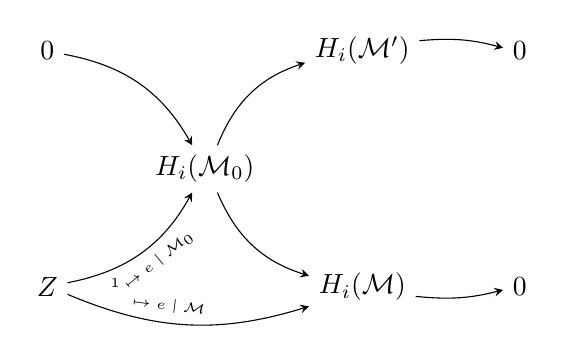
\begin{tikzpicture}
            \draw
                (-2, -1.5) node (B) {\(\mathbb{Z}\)}
                (0, 0) node (C) {\(H_i(\mathcal{M}_0)\)}
                (2, 1.5) node (D) {\(H_i(\mathcal{M}^{\prime})\)}
                (4, 1.5) node (E) {\(0\)}
                (4, -1.5) node (F) {\(0\)}
                (-2, 1.5) node (G) {\(0\)}
                (2, -1.5) node (H) {\(H_i(\mathcal{M})\)}

                (B) edge [bend right = 25, -stealth] node [below = 0.17, pos = 0.3] {\tiny\(1\)} node [sloped, below, pos = 0.56] {\tiny\(\mapsto\eqcl{e\mathrel{|}\mathcal{M}_0}\)} (C)
                (C) edge [bend left = 25, -stealth] (D)
                (D) edge [bend left = 10, -stealth] (E)

                (B) edge [bend right = 20, -stealth] node [sloped, above, pos = 0.41] {\tiny\(\mapsto\eqcl{e\mathrel{|}\mathcal{M}}\)} (H)

                (G) edge [bend left = 25, -stealth] (C)
                (C) edge [bend right = 25, -stealth] (H)
                (H) edge [bend right = 10, -stealth] (F)
                ;
        \end{tikzpicture}
    \end{center}
    Somit gilt 
    \[H_i(\mathcal{M}^{\prime})\cong H_i(\mathcal{M}_0)/\langle\eqcl{e\mathrel{|}\mathcal{M}_0}\rangle\cong H_i(\mathcal{M})/\langle\eqcl{e\mathrel{|}\mathcal{M}}\rangle\,.\]
\end{proof}
Auf \"ahnliche Art und Weise kann der Effekt einer Chirurgie auf die Homotopiegruppen untersucht werden.
\begin{lemma}\label{lem:fund_smaller}
    F\"ur \(k<i<j\) existiert ein Normalteiler \(N\triangleleft\pi_i(\mathcal{M})\) mit \(\eqcl{\mathcal{S}}\in N\) und
    \[\pi_k(\mathcal{M}^{\prime})\cong\pi_k(\mathcal{M})\quad\text{und}\quad\pi_i\left(\mathcal{M}^{\prime}\right)\cong\pi_i(\mathcal{M})/N\,.\]
\end{lemma}
\begin{lemma}\label{lem:odd_surg_effect}
    Chirurgie an einer \textbf{primitiven} Sph\"are \(\mathcal{S}^i\hookrightarrow\mathcal{M}^{2i+1}\) eliminiert die Fundamentalklasse \(\eqcl{\mathcal{S}\mathrel{|}\mathcal{M}}\).
\end{lemma}
\begin{proof}
    Es gilt \(i=j\). Das Diagramm nimmt die folgende Form an:
    \begin{center}
        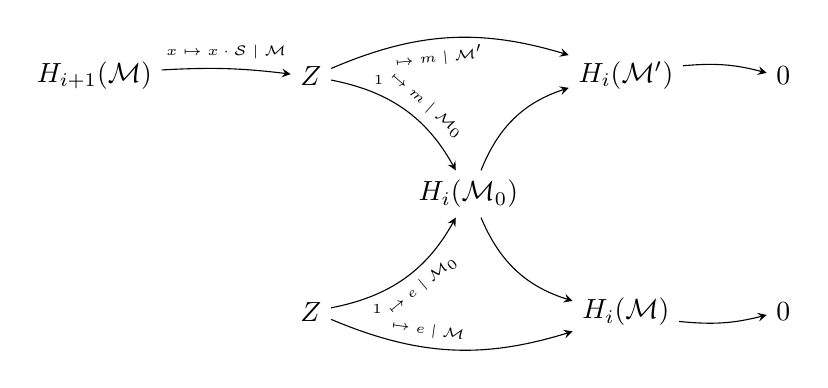
\begin{tikzpicture}
            \draw
                (-4.75, 1.5) node (A) {\(H_{i+1}(\mathcal{M})\)}
                (-2, -1.5) node (B) {\(\mathbb{Z}\)}
                (0, 0) node (C) {\(H_i(\mathcal{M}_0)\)}
                (2, 1.5) node (D) {\(H_i(\mathcal{M}^{\prime})\)}
                (4, 1.5) node (E) {\(0\)}
                (4, -1.5) node (F) {\(0\)}
                (-2, 1.5) node (G) {\(\mathbb{Z}\)}
                (2, -1.5) node (H) {\(H_i(\mathcal{M})\)}

                (A) edge [-stealth, bend left = 5] node [above] {\tiny\(x\mapsto x\cdot\eqcl{\mathcal{S}\mathrel{|}\mathcal{M}}\)} (G)
                (B) edge [bend right = 25, -stealth] node [below = 0.17, pos = 0.29] {\tiny\(1\)} node [sloped, below, pos = 0.56] {\tiny\(\mapsto\eqcl{e\mathrel{|}\mathcal{M}_0}\)} (C)
                (C) edge [bend left = 25, -stealth] (D)
                (D) edge [bend left = 10, -stealth] (E)

                (B) edge [bend right = 20, -stealth] node [sloped, above, pos = 0.39] {\tiny\(\mapsto\eqcl{e\mathrel{|}\mathcal{M}}\)} (H)
                (G) edge [bend left = 20, -stealth] node [sloped, below, pos = 0.45] {\tiny\(\mapsto\eqcl{m\mathrel{|}\mathcal{M}^{\prime}}\)} (D)

                (G) edge [bend left = 25, -stealth] node [above = 0.19, pos = 0.3] {\tiny\(1\)} node [sloped, above, pos = 0.59] {\tiny\(\mapsto\eqcl{m\mathrel{|}\mathcal{M}_0}\)} (C)
                (C) edge [bend right = 25, -stealth] (H)
                (H) edge [bend right = 10, -stealth] (F)
                ;
        \end{tikzpicture}
    \end{center}
    Da die Sph\"are primitiv ist, ist \(H_{i+1}(\mathcal{M})\to\mathbb{Z}\) surjektiv, also \(H_i(\mathcal{M})\cong H_i(\mathcal{M}_0)\). Es folgt 
    \[H_i(\mathcal{M}^{\prime})\cong H_i(\mathcal{M}_0)/\langle\eqcl{e\mathrel{|}\mathcal{M}_0}\rangle\cong H_i(\mathcal{M})/\langle\eqcl{e\mathrel{|}\mathcal{M}}\rangle\,.\]
    F\"ur \(k<i\) hat die Chirurgie keinen Effekt.
\end{proof}
Allgemein l\"asst sich erkennen, dass in diesem Fall 
\[H_i(\mathcal{M}^{\prime})/\langle\eqcl{m\mathrel{|}\mathcal{M}^{\prime}}\rangle\cong H_i(\mathcal{M}_0)/\langle\eqcl{m\mathrel{|}\mathcal{M}_0},\eqcl{e\mathrel{|}\mathcal{M}_0}\rangle\cong H_i(\mathcal{M})/\langle\eqcl{e\mathrel{|}\mathcal{M}}\rangle\]
gilt.
\begin{lemma}\label{lem:even_surg_effect}
    Chirurgie an einer \textbf{primitiven} Sph\"are \(\mathcal{S}^i\hookrightarrow\mathcal{M}^{2i}\) eliminiert die Fundamentalklasse \(\eqcl{\mathcal{S}\mathrel{|}\mathcal{M}}\).
\end{lemma}
\begin{proof}
    Es gilt \(i=j+1\). F\"ur \(k<i-1\) hat die Chirurgie keinen Effekt. Der interessante Anteil des Diagramms ist von der Form:
    \begin{center}
        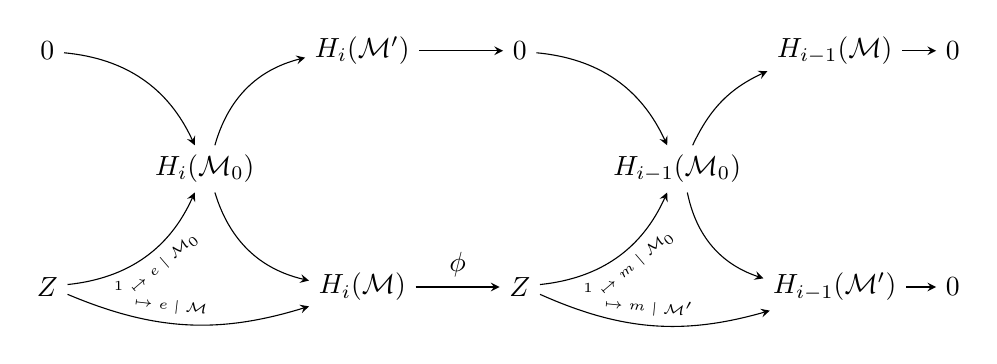
\begin{tikzpicture}
            \draw
                (-2, -1.5) node (B) {\(\mathbb{Z}\)}
                (0, 0) node (C) {\(H_i(\mathcal{M}_0)\)}
                (2, 1.5) node (D) {\(H_i(\mathcal{M}^{\prime})\)}
                (4, 1.5) node (E) {\(0\)}
                (-2, 1.5) node (G) {\(0\)}
                (2, -1.5) node (H) {\(H_i(\mathcal{M})\)}
                (4, -1.5) node (I) {\(\mathbb{Z}\)}
                (6, 0) node (J) {\(H_{i-1}(\mathcal{M}_0)\)}
                (8, 1.5) node (K) {\(H_{i-1}(\mathcal{M})\)}
                (8, -1.5) node (L) {\(H_{i-1}(\mathcal{M}^{\prime})\)}
                (9.5, -1.5) node (M) {\(0\)}
                (9.5, 1.5) node (N) {\(0\)}
                
                (B) edge [bend right = 30, -stealth] node [below = 0.17, pos = 0.31] {\tiny\(1\)} node [sloped, below, pos = 0.57] {\tiny\(\mapsto\eqcl{e\mathrel{|}\mathcal{M}_0}\)} (C)
                (B) edge [bend right = 20, -stealth] node [sloped, above, pos = 0.42] {\tiny\(\mapsto\eqcl{e\mathrel{|}\mathcal{M}}\)} (H)
                (C) edge [bend left = 30, -stealth] (D)
                (D) edge [-stealth] (E)
                (E) edge [bend left = 30, -stealth] (J)
                (J) edge [bend right = 30, -stealth] (L)
                (L) edge [-stealth] (M)

                (G) edge [bend left = 30, -stealth] (C)
                (C) edge [bend right = 30, -stealth] (H)
                (H) edge [-stealth] node [above] {\(\phi\)} (I)
                (I) edge [bend right = 30, -stealth] node [below = 0.17, pos = 0.29] {\tiny\(1\)} node [sloped, below, pos = 0.57] {\tiny\(\mapsto\eqcl{m\mathrel{|}\mathcal{M}_0}\)}  (J)
                (I) edge [bend right = 20, -stealth] node [sloped, above, pos = 0.47] {\tiny\(\mapsto\eqcl{m\mathrel{|}\mathcal{M}^{\prime}}\)}  (L)
                (J) edge [bend left = 20, -stealth] (K)
                (K) edge [-stealth] (N)
                ;
        \end{tikzpicture}
    \end{center}
    Wegen der Primitivit\"at ist \(\phi\colon H_i(\mathcal{M})\to\mathbb{Z},\,x\mapsto x\cdot\eqcl{\mathcal{S}\mathrel{|}\mathcal{M}}\) ein Epimorphismus, also folgt
    \[H_{i-1}(\mathcal{M}^{\prime})\cong H_{i-1}(\mathcal{M}_0)\cong H_{i-1}(\mathcal{M})\,.\]
    Weiter gilt
    \[H_i(\mathcal{M}^{\prime})\cong H_i(\mathcal{M}_0)/\langle\eqcl{e\mathrel{|}\mathcal{M}_0}\rangle\cong\ker\phi/\langle\eqcl{e\mathrel{|}\mathcal{M}}\rangle\,.\]
    Wegen \(\ker\phi\subseteq H_i(\mathcal{M})\) wird \(\eqcl{\mathcal{S}\mathrel{|}\mathcal{M}}\) eliminiert, wo\-m\"og\-lich mehr.
\end{proof}

\section{Gerahmte Chirurgie}
    Sei \({n=i+j+1}\), \(\mathcal{M}^n\) eine \(\pi\)-Mannigfaltigkeit und \(\Psi\colon\underline{\mathbb{D}}^{j+1}\hookrightarrow\mathring{\mathcal{M}}\) eine beliebige Anklebeeinbettung. Bezeichne durch \(\mathcal{S}:=\Psi(\mathbb{S}^i\times\mathbf{0})\) die Anklebesph\"are. Die naive Chirurgie bez\"uglich dieser Daten kann unter Umst\"anden eine Mannigfaltigkeit liefern, die nicht stabil parallelisierbar ist. Um dem beizukommen, reicht es aus, die Anklebeeinbettungen mithilfe von einer glatten Funktion \(\gamma\colon\mathbb{S}^i\to\operatorname{SO}(j+1)\) informiert zu \textit{verdrehen}. 

Sei \(F\) eine stabile Rahmung von \(\mathcal{M}\). Eine stabile Rahmung \(\overline{F}\) auf \(\mathcal{M}\multimap\mathbb{S}^i\) induziert offenbar eine Rahmung von \(\mathcal{M}\setminus\mathcal{S}\). Ist diese induzierte stabile Rahmung zu \(F\) homotop, hei\ss e die Chirurgie gerahmt. 

Zu einer Folge gerahmter Mannigfaltigkeiten \((\mathcal{M}_i,F_i)\) mit \(1\leq i\leq m\), sodass \(\mathcal{M}_{i+1}\) durch gerahmte Chirurgie aus \(\mathcal{M}_i\) erhalten werden kann, hei\ss en \(\mathcal{M}_1\) und \(\mathcal{M}_m\) zueinander \textbf{\(\chi\)-\"aquivalent}. Diese Relation ist offenbar reflexiv und transitiv. Sie ist symmetrisch, denn wird an der transversalen Sph\"are einer \(i\)-Chirurgie eine \(j\)-Chirurgie durchgef\"uhrt, ergibt sich erneut die originale Mannigfaltigkeit. Derart ist also eine \"Aquivalenz\-re\-la\-tion definiert.

\subsection{Strategie der Berechnung von \texorpdfstring{\(\Theta_k\)}{TEXT}}
    Sei \(P^k\) die Menge der \(\chi\)-\"Aquivalenzklassen gerahmter Mannigfaltigkeiten, die Homotopiesph\"aren beranden. Diese sei mit der verbundenen Randsumme versehen, sodass \(P^k\) die Struktur eines kommutativen Monoiden erh\"alt. Da Chirurgie stets am Inneren vorgenommen wird, hat diese keinen Einfluss auf den Rand, sodass \(\chi\)-\"aquivalente, gerahmte Mannigfaltigkeiten stets diffeomorphe R\"ander besitzen. Es folgt, dass der Randoperator \(\partial\colon P_k\to\Theta_k\) ein wohldefinierter Homomorphismus ist. Die Berechnung dieser Untergruppe ist der erste Schritt in der Berechnung von \(\Theta_k\). Es existiert die offensichtliche exakte Folge
    \[0\to\ker\partial\to P^k\mathop{\longrightarrow}^{\partial}\partial P^k\to0\,.\]
    Der Kern besteht hierbei gerade aus all den \(\chi\)-\"Aquivalenzklassen gerahmter Mannigfaltigkeiten, deren Rand zu der Standardsph\"are diffeomorph ist. Um die Gruppe \(\partial P^k\subseteq\Theta_k\) zu berechnen wird eine Mannigfaltigkeit aus \(P^k\) nun so lange durch gerahmte Chirurgie bearbeitet, bis sie m\"oglichst simpel ist. 

\subsection{Rahmbarkeit und Reparametrisierung}
    Sei erneut \({n=i+j+1}\), \((\mathcal{M}^n,F)\) eine stabil gerahmte Mannigfaltigkeit und \({\Psi\colon\underline{\mathbb{D}}^{j+1}\hookrightarrow\mathring{\mathcal{M}}}\) eine Anklebeeinbettung. Es soll untersucht werden, wann eine Verklebung mit der Standard-Sph\"are \((\mathbb{S}^n,E\)) eine stabil gerahmte Mannigfaltigkeit ergibt. Zun\"achst ist \(F(p)\) eine Basis von \({T_p\mathcal{M}\oplus\mathbb{R}}\) und \(E(p)\) eine Basis von \({T_p\mathbb{S}^n\oplus\mathbb{R}}\). Wird eine Umgebung von \({\mathbb{S}^i\subseteq\mathbb{S}^n}\) mit dem Definitionsbereich von \(\Psi\) identifiziert, ist die Einh\"angung des Differentials von \(\Psi\) eine Funktion
    \[S(\dx_p\Psi)\colon T_p\mathbb{S}^n\oplus\mathbb{R}\to T_{\Psi(p)}\mathcal{M}\oplus\mathbb{R}\,.\]
    Derart wird \(E\) zu einer stabilen Rahmung von \(\im\Psi\subseteq\mathcal{M}\) transportiert. Bezeichne jene Rahmung durch \(\dx\Psi(E)\). Sei \(\sigma(F,\Psi)\) der Rahmenwechsel von \(\dx\Psi(E)\) zu \(F\) auf \(\Psi(\mathbb{S}^i\times\mathbf{0})\). Da der Basiswechsel der transportierten Basis zu \(F\) gerade die Abbildungsmatrix von \(S(\dx_p\Psi)\) bez\"uglich \(E\) und \(F\) ist, gilt mit \(q=\Psi(p,0)\)
    \[\sigma(F,\Psi)\colon\mathbb{S}^i\to\operatorname{GL}^+(n+1),\,p\mapsto M_{F(q)}^{E(p,0)}\left(S(\dx_{(p,0)}\Psi)\right)\,.\]
    Derart wird ein Element \({\mathfrak{o}(F,\Psi):=\eqcl{\sigma(F,\Psi)}\in\pi_i(\operatorname{SO}(n+1))}\) definiert. Wegen folgendem Lemma kann \(\mathfrak{o}(F,\Psi)\) als Obstruktion betrachtet werden.
    \begin{lemma}\label{lem:nullhom_frame}
        Sei \((\mathcal{M},F)\) eine gerahmte Mannigfaltigkeit und \(\Psi\colon\underline{\mathbb{D}}^{j+1}\hookrightarrow\mathring{\mathcal{M}}\) eine An\-kle\-be\-ein\-bet\-tung. Dann ist die Verklebung von \((\mathcal{M},F)\) mit \((\mathbb{S}^n,E)\) genau dann gerahmt, wenn \({\mathfrak{o}\left(F,\Psi\right)=0}\) gilt.
    \end{lemma}
    \begin{proof}
        Sei \({(\mathcal{M}+\mathbb{S}^n,\overline{F})}\) zun\"achst gerahmt, sodass \(\overline{F}\) und \(F\) auf \({\mathcal{M}\setminus\Psi(\mathbb{S}^i\times\mathbf{0})}\) homotop sind. Der Rahmenwechsel von \(\overline{F}\) zu \(\dx\Psi(E)\) auf \(\Psi(\mathbb{S}^i\times\mathbb{S}^j)\) ist offenbar konstant, also ist der Rahmenwechsel von \(F\) zu \(\dx\Psi(E)\) auf \(\Psi(\mathbb{S}^i\times\mathbb{S}^j)\) nullhomotop. Es l\"asst sich leicht zeigen, dass dies genau dann der Fall ist, wenn eine nullhomotope Fortsetzung auf \({\Psi(\mathbb{S}^i\times\mathbb{D}^{j+1})\simeq\Psi(\mathbb{S}^i\times\mathbf{0})}\) existiert. Es folgt \({\mathfrak{o}\left(F,\Psi\right)=0}\).

        Sei umgekehrt \({\mathfrak{o}\left(F,\Psi\right)=0}\), der Rahmenwechsel von \(F\) zu \(\dx\Psi(E)\) auf der Anklebesph\"are sei also nullhomotop. Da diese ein Deformationsretrakt von \(\im\Psi\) ist, ist auch der Rahmenwechsel auf \(\im\Psi\) nullhomotop. Eine Nullhomotopie \({\im\Psi\times\mathbb{I}\to\operatorname{GL}^+(n+1)}\) zu der Identit\"at kann mithilfe der Homotopie\-er\-wei\-te\-rungs\-ei\-gen\-schaft zu einer Homotopie \({H\colon\mathcal{M}\times\mathbb{I}\to\operatorname{GL}^+(n+1)}\) fortgesetzt werden. Dann ist durch \({\overline{F}(p):=H(p,1)\cdot F(p)}\) eine Rahmung von \(\mathcal{M}\) definiert, die einerseits zu \(F\) homotop ist, und andererseits auf \(\im\Psi\) mit \(\dx\Psi(E)\) \"uber\-ein\-stimmt. Zusammen mit \(E\) induziert \(\overline{F}\) eine Rahmung auf \(\mathcal{M}+\mathbb{S}^n\).
    \end{proof}
    Sei \({n=i+j+1}\), \(\mathcal{M}\) eine Mannigfaltigkeit und \(\Psi\colon\underline{\mathbb{D}}^{j+1}\hookrightarrow\mathring{\mathcal{M}}\) eine Anklebe\-ein\-bet\-tung. Zu einer glatten Funktion \(\gamma\colon\mathbb{S}^{i-1}\to\operatorname{SO}(j+1)\) l\"asst sich der Vektorb\"undel\-auto\-mor\-phis\-mus
    \[\Gamma\colon\underline{\mathbb{D}}^{j+1}\to\underline{\mathbb{D}}^{j+1},\,(x,y)\mapsto\left(x,\gamma(x)\cdot y\right)\]
    definieren. Dann l\"asst sich die reparametrisierte Chirurgie mithilfe von \(\Psi\Gamma\) bilden. Besonders interessant ist hierbei der Effekt einer Reparametrisierung auf die Obstruktion der stabilen Parallelisierbarkeit. In folgendem Lemma bezeichne \(S^k\colon\operatorname{SO}(m)\to\operatorname{SO}(m+k)\) die \(k\)-fach iterierte Einh\"angung.
    \begin{lemma}\label{lem:reparam_eq}
        Sei \({n=i+j+1}\), \((\mathcal{M}^n,F)\) eine gerahmte Mannigfaltigkeit, \(\Psi\colon\underline{\mathbb{D}}^{j+1}\hookrightarrow\mathring{\mathcal{M}}\) eine Anklebeeinbettung und \(\gamma\colon\mathbb{S}^i\to\operatorname{SO}(j+1)\) glatt. Dann gilt die Gleichung
        \begin{equation}\label{eq:reparam_eq}
            \mathfrak{o}\left(F,\Psi\Gamma\right)=\mathfrak{o}\left(F,\Psi\right)+S_*^{i+1}\eqcl{\gamma}\in\pi_i\left(\operatorname{SO}(n+1)\right)\,.
        \end{equation}
    \end{lemma}
    \begin{proof}
        F\"ur das Differential
        \[\dx_{(p,q)}\Gamma\colon T_{(p,q)}(\mathbb{S}^i\times\mathbb{D}^{j+1})\to T_{(p,q)}(\mathbb{S}^i\times\mathbb{D}^{j+1})\]
        bez\"uglich der Standardbasis \((e_k)_{1\leq k\leq n}=E(p,q)\) gilt
        \[J\Gamma(p,q)=M_{E(p,q)}^{E(p,q)}\left(\dx_{(p,q)}\Gamma\right)=\begin{pmatrix}
            I_i & J\gamma(p)\cdot q\\
            0 & \gamma(p)
        \end{pmatrix}\in\operatorname{GL}^+(n)\,.\]
        Folglich gilt \({J\Gamma(p,0)=S^i\gamma(p)\in\operatorname{SO}(n)}\). F\"ur \(p\in\mathbb{S}^i\) folgt
        \begin{align*}
            \sigma(F,\Psi\Gamma)(p)&\overeq{Def}M_{F(q)}^{E(p,0)}\left(S(\dx_{(p,0)}(\Psi\Gamma))\right)\\
            &=M_{F(q)}^{E(p,0)}\left(S(\dx_{\Gamma(p,0)}\Psi)\circ S(\dx_{(p,0)}\Gamma)\right)\\
            &=M_{F(q)}^{E(p,0)}\left(S(\dx_{(p,0)}\Psi)\right)\cdot M_{E(p,0)}^{E(p,0)}\left(S(\dx_{(p,0)}\Gamma)\right)\\
            &=\sigma(F,\Psi)(p)\cdot S\left(J\Gamma(p,0)\right)\\
            &=\sigma(F,\Psi)(p)\cdot S^{i+1}\gamma(p)\,.
        \end{align*}
        Dies zeigt \(\mathfrak{o}\left(F,\Psi\Gamma\right)=\mathfrak{o}\left(F,\Psi\right)+S_*^{i+1}\eqcl{\gamma}\).
    \end{proof}
    Insbesondere hat Reparametrisierung mit \(\eqcl{\gamma}\in\ker S_*^{i+1}\) keine Auswirkung auf stabile Parallelisierbarkeit.
    \newpage
    \begin{theorem}\label{thm:surg_framable}
        Sei \(n=i+j+1\), \((\mathcal{M}^n,F)\) eine gerahmte Mannigfaltigkeit und \(\mathcal{S}^i\) eine eingebettete Sph\"are mit trivialem Normalenb\"undel. Gilt \(i\leq j\), l\"asst sich an \(\mathcal{S}\) eine gerahmte Chirurgie durch\-f\"uh\-ren.
    \end{theorem}
    \begin{proof}
        Sei \(\Psi\colon\underline{\mathbb{D}}^{j+1}\to\mathring{\mathcal{M}}\) eine beliebige Anklebeabbildung, sodass die Obstruktion \(\mathfrak{o}(F,\Psi)\in\pi_i\left(\operatorname{SO}(n+1)\right)\) definiert ist. Aus der Annahme folgt, dass der von der \(i\)-fach iterierten Einh\"angung induzierte Homomorphismus
        \[S_*^{i+1}\colon\pi_i\left(\operatorname{SO}(j+1)\right)\to\pi_i\left(\operatorname{SO}(n+1)\right)\]
        surjektiv ist, es existiert also ein \(\eqcl{\gamma}\in\pi_i\left(\operatorname{SO}(j+1)\right)\) mit einem glatten Re\-pr\"a\-sen\-tan\-ten \(\gamma\), sodass f\"ur die Reparametrisierung \(\Gamma\) gem\"a\ss{} Lemma \ref{lem:reparam_eq}
        \[\mathfrak{o}\left(F,\Psi\Gamma\right)=\mathfrak{o}\left(F,\Psi\right)+S_*^{i+1}\eqcl{\gamma}=0\]
        gilt. Gem\"a\ss{} Lemma \ref{lem:nullhom_frame} ist eine Chirurgie an \(\mathcal{S}\) mittels \(\Psi\Gamma\) gerahmt.
    \end{proof}

    \begin{theorem}\label{thm:srg_conn}
        Eine gerahmte Mannigfaltigkeit \((\mathcal{M}^n,F)\) mit \({n\geq2k}\) ist zu einer \({(k-1)}\)-zu\-sam\-men\-h\"angen\-den gerahmten Mannigfaltigkeit \(\chi\)-\"aquivalent.
    \end{theorem}
    \begin{proof}
        Es wird Induktion \"uber \(k\) gef\"uhrt. Durch \(0\)-Chirurgie kann \(\mathcal{M}\) als zusammenh\"angend angenommen werden. Sei \(\mathcal{M}\) nun bereits \((k-2)\)-zusammen\-h\"angend. Dann kann ein beliebiges Element in \(\pi_{k-1}(\mathcal{M})\) durch eine Einbettung \(\mathbb{S}^{k-1}\hookrightarrow\mathcal{M}\) repr\"asentiert werden. Da die Bildsph\"are wegen Satz \ref{thm:vec_dim_triv} ein triviales Normalenb\"undel besitzt, kann Chirurgie an ihr durchgef\"uhrt werden. Mithilfe von Satz \ref{thm:surg_framable} ergibt dies erneut eine gerahmte Mannigfaltigkeit \(\mathcal{M}^{\prime}\). Wegen Lemma \ref{lem:fund_smaller} ist \(\pi(\mathcal{M}^{\prime})\) echt kleiner als \(\pi(\mathcal{M})\). Endlich viele Schritte f\"uhren zu einer \((k-1)\)-zusammen\-h\"angen\-den Mannigfaltigkeit.
    \end{proof}

\subsection{Gerahmte Henkel}
    Die vorangegangenen S\"atze gelten in \"ahnlicher Art und Weise, wenn mit Henkeln anstatt mit Chirurgie gearbeitet wird. Ein zu Lemma \ref{lem:nullhom_frame} nahezu analoger Beweis ergibt:
    \begin{lemma}
        Sei \((\mathcal{W},F)\) eine gerahmte Mannigfaltigkeit und \(\Psi\colon\underline{\mathbb{D}}^{j+1}\hookrightarrow\partial\mathcal{W}\) eine An\-kle\-be\-ein\-bet\-tung und \(\tilde{\Psi}\colon\underline{\mathbb{D}}^{j+1}\hookrightarrow\mathcal{W}\) eine Fortsetzung. Dann ist die Verklebung von \((\mathcal{W},F)\) mit \((\mathbb{D}^n,E)\) genau dann rahmbar, wenn \({\mathfrak{o}\left(F|_{\partial\mathcal{W}},\Psi\right)=0}\) gilt.
    \end{lemma}
    Die Obstruktionen der Rahmbarkeit von \(\mathcal{W}\multimap\mathbb{D}^{i+1}\) und \(\partial\mathcal{W}\multimap\mathbb{S}^i\) stimmen also \"uberein. Eine Reparametrisierung ist nun eine Abbildung
    \[\tilde{\Gamma}\colon\underline{\mathbb{D}}^j\times\mathbb{R}_+\to\underline{\mathbb{D}}^j\times\mathbb{R}_+,\,(x,y,t)\mapsto\left(x,\gamma(x)\cdot y,t\right)\,,\]
    und setzt damit die Reparametrisierung der Chirurgie an \(\partial\mathcal{W}\) trivial fort. F\"ur das folgende ist noch folgendes Lemma wichtig.
    \begin{lemma}\label{lem:smoothing_pi}
        Zu einer gerahmten Mannigfaltigkeit \(\mathcal{M}^n\) und \({i\leq j}\) existiert eine gerahmte Man\-nig\-faltig\-keit \(\mathcal{W}^{n+1}\) mit
        \[\partial\mathcal{W}\cong\mathcal{M}\mathop{+}^{\partial\mathcal{M}}\left(\mathcal{M}\multimap\mathbb{S}^i\right)\,.\]
    \end{lemma}
    \begin{proof}
        Sei \(\mathcal{W}\subseteq\mathcal{M}\times\mathbb{I}\) mit 
        \[\partial\mathcal{W}\cong\mathcal{M}\mathop{+}^{\partial\mathcal{M}}\mathcal{M}\,.\]
        gem\"a\ss{} Lemma \ref{lem:smooth_man}. Da die stabile Rahmung von \(\mathcal{M}\) eine Rahmung von \({\mathcal{M}\times\mathbb{R}}\) induziert, induziert diese auch eine Rahmung von \(\mathcal{W}\). Wegen \(i\leq j\) kann an \(\mathcal{W}\) derart ein gerahmter Henkel angebracht werden, dass die resultierende Mannigfaltigkeit dem Lemma  gen\"ugt.
    \end{proof}

\section{Probleme in gerader Dimension}
    Sei \(\mathcal{M}^{2k}\) eine \((k-1)\)-zusammenh\"angende \(\pi\)-Mannigfaltigkeit mit \(k\geq3\), deren Rand entweder leer oder eine Homotopiesph\"are ist. Um \(\mathcal{M}\) durch Chirurgie in eine \(k\)-zusammenh\"angende \(\pi\)-Mannigfaltigkeit zu \"uberf\"uhren m\"ussen einige Hindernisse beachtet werden. Einerseits muss das Normalenb\"undel einer eingebetteten \(k\)-Sph\"are nicht unbedingt trivial sein, andererseits ist nicht jede Sph\"are primitiv und vereinfacht somit nicht unbedingt die Homologie. In diesem Fall ist die mittlere Homologiegruppe \(H_k(\mathcal{M})\) jedoch frei, sodass keine Komplikationen durch Torsion auftreten. 
\begin{lemma}\label{lem:middle_free}
    Sei \(\mathcal{M}^{2k}\) mit \({H_k(\partial\mathcal{M})=H_{k-1}(\partial\mathcal{M})=0}\) derart, dass \(H_{k-1}(\mathcal{M})\) frei ist. Dann ist auch \(H_k(\mathcal{M})\) frei.
\end{lemma}
\begin{proof}
    Aus der Annahme an den Rand folgt, dass \(q^*\colon H_k(\mathcal{M})\to H_k(\mathcal{M},\partial\mathcal{M})\) ein Isomorphismus ist. Sei \(T_k\) die Torsionsuntergruppe von \(H_k(\mathcal{M})\). Es folgt
    \[H_k(\mathcal{M})\mathop{\cong}^{q^*}H_k(\mathcal{M},\partial\mathcal{M})\overcong{P.D.}H^k(\mathcal{M})\overcong{U.K.}\operatorname{Hom}(H_k(\mathcal{M}),\mathbb{Z})\cong H_k(\mathcal{M})/T_k\,.\]
    Somit muss \(T_k=0\), und \(H_k(\mathcal{M})\) frei sein.
\end{proof}

\subsection{Repr\"asentierende Sph\"aren}
    Sei \(\mathcal{M}^{2k}\) eine \((k-1)\)-zusammenh\"angende \(\pi\)-Mannigfaltigkeit und \(x\in H_k(\mathcal{M})\). Gem\"a\ss{} dem Satz von Hurewicz ist
    \[h\colon\pi_k(\mathcal{M})\to H_k(\mathcal{M}),\,\eqcl{\gamma}\mapsto\gamma_*\big(\eqcl{\mathbb{S}^k}\big)\]
    ein Isomorphimus. Es existiert also eine bis auf Homotopie eindeutig bestimmte Funktion \(\phi\colon\mathbb{S}^k\to\mathcal{M}\) mit \(\phi_*\eqcl{\mathbb{S}^k}=x\). Aufgrund eines Satzes von Haelfiger (\cite{haefliger1961differentiable} Satz 1) kann f\"ur \(k\geq3\) angenommen werden dass \(\phi\) eine Einbettung ist. Bezeichne die eingebettete Sph\"are durch \(\mathcal{S}(x)\). Diese ist f\"ur \(k\geq4\) bis auf Isotopie eindeutig bestimmt, sodass sich die Homotopieklasse der Kupplungsfunktion des Normalenb\"undels von \(\mathcal{S}(x)\) in \(\mathcal{M}\) betrachten l\"asst. F\"ur \(k\geq4\) ist also die Funktion
    \[\alpha\colon H_k(\mathcal{M})\to\pi_{k-1}(\operatorname{SO}(k)),\,x\mapsto\eqcl{\nu(\mathcal{S}(x))}\]
    wohldefiniert. Aufgrund von \(\pi_2(\operatorname{SO}(3))=0\) l\"asst sich \(\alpha\) auch f\"ur \(k=3\) definieren. Es folgt nun aus vorherigen \"Uberlegungen \ref{subsec:stable_normal_bundle}, das \(\alpha(x)\) ein ganzzahliges Vielfaches der Kupplungsfunktion des Normalenb\"undels ist, und
    \begin{equation}\label{eq:alpha_kernel}
        \alpha(x)\in\ker S_*\cong\begin{cases}
            \mathbb{Z} & k=2m\\
            \mathbb{Z}_2 & k=2m+1\notin\{3,7\}\\
            0 & k\in\{3,7\}
        \end{cases}
    \end{equation}
    gilt. Die Entscheidung, wann das Normalenb\"undel trivial ist, h\"angt also von der Parit\"at von \(k\) ab.

\subsection{Symplektische Basen}
    \begin{definition}[Schwach symplektische Basis]
        Sei \(M^{2k}\) ein freier \(R\)-Modul. Eine Basis \((e_i,f_i)_{1\leq i\leq k}\) von \(M\), hei\ss e schwach symplektisch bez\"uglich einer Bilinearform \(\beta\colon M\otimes M\to R\), falls
        \[\beta(e_i,f_j)=\delta_{ij}\quad\text{und}\quad\beta(e_i,e_j)=\beta(f_i,f_j)=0\quad\text{f\"ur alle}\quad1\leq i,j\leq k\,.\]
    \end{definition}
    Ist \(\beta\) schiefsymmetrisch, hei\ss e sie symplektisch. Die Signifikanz dieser Basen liegt unter anderem in folgendem Satz.
    \begin{theorem}\label{thm:even_symp_ann}
        Sei \(k\geq3\) und \(\mathcal{M}^{2k}\) eine \((k-1)\)-zusammenh\"angende, gerahmte Mannigfaltigkeit, deren Rand leer oder eine Homotopiesph\"are ist, sodass \(H_k(\mathcal{M})\) eine schwach symplektische Basis \(e_i,f_i\) mit \(\alpha(e_i)=0\) besitzt. Dann kann \(H_k(\mathcal{M})\) durch gerahmte Chirurgie vernichtet werden.
    \end{theorem}
    \begin{proof}
        Da \(e_1\) ein triviales Normalenb\"undel besitzt, kann Chirurgie an \(e_1\) durchgef\"uhrt werden. Sei \(\mathcal{S}\) die Anklebesph\"are und \(\mathcal{M}^{\prime}\) die resultierende Mannigfaltigkeit. Da die \(e_i,f_i\) eine schwach symplektische Basis bilden, ist \(e_1\) primitiv, und es gilt f\"ur
        \[\phi\colon H_i(\mathcal{M})\to\mathbb{Z},\,x\mapsto x\cdot e_1\]
        gerade \(\ker\phi=H_i(\mathcal{M})/\langle f_1\rangle\). Aus Satz \ref{lem:even_surg_effect} folgt
        \[H_i(\mathcal{M}^{\prime})\cong\ker\phi/\langle e_1\rangle\cong H_i(\mathcal{M})/\langle e_1,f_1\rangle\,.\]
        \"Uber Transversalit\"at kann angenommen werden, dass die Bilder \(e_i^{\prime},f_i^{\prime}\in H_i(\mathcal{M}^{\prime})\) durch Sph\"aren in \(\mathcal{M}\setminus\mathcal{S}\) repr\"asentiert werden, sodass sich die Schnittzahlen nicht \"andern und die \(e_i^{\prime},f_i^{\prime}\) erneut eine symplektische Basis mit \(\alpha(e_i^{\prime})=0\) bilden. Die Aussage folgt rekursiv.
    \end{proof}
    Es wird im Folgenden noch eine weitere symplektische Basis \({e_i,f_i\in H_k(\partial\mathcal{W})}\) ben\"otigt werden, wobei alle \(e_i\) im Kern der Inklusion \({\partial\mathcal{W}\hookrightarrow\mathcal{W}^{2k+1}}\) liegen. Hierbei sei stets an den Torus erinnert. Es gilt \({H_1(\mathbb{S}^1\times\mathbb{S}^1)\cong\mathbb{Z}\oplus\mathbb{Z}}\), wobei die Erzeuger eine symplektische Basis bilden. Eines der Elemente liegt im Kern der Inklusion \(\mathbb{S}^1\times\mathbb{S}^1\hookrightarrow\mathbb{D}^2\times\mathbb{S}^1\) des Torus als Rand des Volltorus. Es wird folgendes Lemma ben\"otigt. Im folgenden Satz bezeichne \(\operatorname{Ad}\) zu einem K\"orper \(\mathbb{K}\) die Abbildung
    \[\operatorname{Ad}\colon H_i(\partial\mathcal{W};\mathbb{K})\to\operatorname{Hom}(H_{n-i}(\partial\mathcal{W};\mathbb{K}),\mathbb{K}),\,x\mapsto x\cdot(\mathrel{-})\,.\]
    \begin{lemma}\label{lem:inter_annihilates}
        Sei \(\mathbb{K}\) ein K\"orper, \(\mathcal{W}^{2k+1}\) eine Mannigfaltigkeit, 
        \[A_i:=\ker\left(\iota_*\colon H_i(\partial\mathcal{W};\mathbb{K})\to H_i(\mathcal{W};\mathbb{K})\right)\]
        und \(R\colon\operatorname{Hom}(H_{n-i}(\partial\mathcal{W};\mathbb{K}),\mathbb{K})\to\operatorname{Hom}(A_{n-i},\mathbb{K})\) die Einschr\"ankung, dann ist der Kern von \(F:=R\circ\operatorname{Ad}\) gerade \(A_i\).
    \end{lemma}
    \begin{proof}
        Ein \(x\in H_i(\partial\mathcal{W};\mathbb{K})\) liegt genau dann in \(\ker F\), wenn \({(A_{n-i})\cdot x=0}\) ist. Betrachte das bis auf Vorzeichen kommutive Diagramm
        \begin{center}
            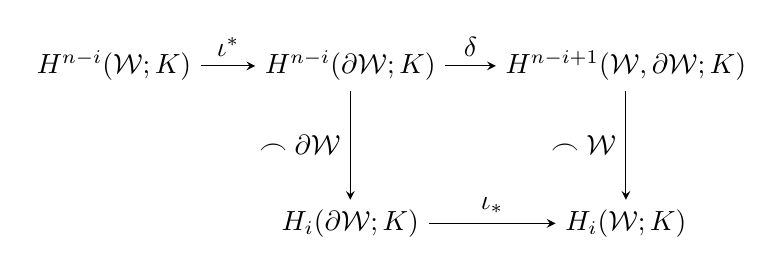
\begin{tikzpicture}
                \draw 
                    (-3, 0) node (A) {\(H^{n-i}(\mathcal{W};\mathbb{K})\)}
                    (0, 0) node (B) {\(H^{n-i}(\partial\mathcal{W};\mathbb{K})\)}
                    (3.5, 0) node (C) {\(H^{n-i+1}(\mathcal{W},\partial\mathcal{W};\mathbb{K})\)}
                    (0, -2) node (E) {\(H_i(\partial\mathcal{W};\mathbb{K})\)}
                    (3.5, -2) node (F) {\(H_i(\mathcal{W};\mathbb{K})\)}

                    (A) edge [-stealth] node [above] {\(\iota^*\)} (B)
                    (B) edge [-stealth] node [above] {\(\delta\)} (C)
                    (B) edge [-stealth] node [left] {\(\frown\eqcl{\partial\mathcal{W}}\)} (E)
                    (C) edge [-stealth] node [left] {\(\frown\eqcl{\mathcal{W}}\)} (F)
                    (E) edge [-stealth] node [above] {\(\iota_*\)} (F)
                    ;
            \end{tikzpicture}
        \end{center}
        F\"ur \(x\in H_i(\partial\mathcal{W};\mathbb{K})\) gilt
        \[(A_{n-i})\cdot x=\langle(\ker\iota_*)^*,x\rangle=\langle\im\iota^*,x\rangle=\langle H^{n-i}(\mathcal{W};\mathbb{K}),\iota_*x\rangle\,.\]
        Also liegt \(x\) genau dann im Kern von \(F\), wenn \(\langle H^{n-i}(\mathcal{W};\mathbb{K}),\iota_*x\rangle=0\) ist. Da \(\mathbb{K}\) ein K\"orper und die Kronecker-Paarung nicht degeneriert ist, ist dies zu \(x\in\ker\iota_*=A_i\) \"aquivalent.
    \end{proof}
    Die Beweisidee entstammt hierbei \cite{tomdieck2008algebraic} Proposition 18.7.5. Es ergibt sich somit \(\dim_{\mathbb{K}}A_{n-i}=\dim_{\mathbb{K}}H_i(\partial\mathcal{W};\mathbb{K})-\dim_{\mathbb{K}}A_i\), insbesondere also
    \begin{equation}\label{eq:ker_incl_dim}
        \dim_{\mathbb{K}}H_k(\partial\mathcal{W};\mathbb{K})=2\dim_{\mathbb{K}}A_k=2\dim_{\mathbb{K}}\ker\iota_*\,.
    \end{equation}
    Beachte, dass die Forderung, dass \(\mathbb{K}\) ein K\"orper n\"otig ist, da \(H_k(\mathcal{W})\) Torsion aufweisen k\"onnte. In diesem Fall k\"onnte die Kronecker-Paarung degeneriert sein. Wird Torsion herausgeteilt, gilt der vorherige Satz auch f\"ur \(\mathbb{Z}\)-Koeffizienten. Siehe etwa \cite{hatcher2002algebraic} Proposition 3.38. F\"ur die Abbildung
    \[\iota_*^{\prime}\colon H_k(\partial\mathcal{W})\xrightarrow{\iota_*}H_k(\mathcal{W})\xrightarrow{p}H_k(\mathcal{W})/T_k(\mathcal{W})\]
    gilt also gerade \(2\operatorname{Rang}\ker\iota_*^{\prime}=\operatorname{Rang}H_k(\partial\mathcal{W})\). Da das Herausteilen der Torsion keinen Einfluss auf den Rang hat, gilt \(\operatorname{Rang}\ker\iota_*=\operatorname{Rang}\ker\iota_*^{\prime}\) und
    \begin{equation}
        \operatorname{Rang}H_k(\partial\mathcal{W})=2\operatorname{Rang}\ker\iota_*\,.
    \end{equation}

    \begin{theorem}\label{thm:symp_base_ann}
        Sei \(k\) ungerade und \(\mathcal{M}^{2k}\) eine Mannigfaltigkeit mit \(H_k(\partial\mathcal{M})=H_{k-1}(\partial\mathcal{M})=0\). Dann existiert eine symplektische Basis von \(H_k(\mathcal{M})\) mit \(e_i\in\ker\iota_*\).
    \end{theorem}
    \begin{proof}
        Da \(k\) ungerade ist, besitzt \(H_k(\mathcal{M})\) geraden Rang, und es gilt \(x\cdot x=0\) f\"ur alle \(x\in H_k(\mathcal{M})\). Sei \(e_1\in\ker\iota_*\). Da die Schnittform unimodular ist, existiert ein \(f_1\in H_k(\mathcal{M})\) mit \(e_1\cdot f_1=1\). Da die Schnittform unimodular ist, spaltet \(f_i\) von \(H_k(\mathcal{M})\) und \(e_i\) von \(\ker\iota_*\) ab, sodass die Aussage rekursiv folgt.
    \end{proof}